%
%  Vincent Yannello
%
\documentclass[12pt,fullpage]{article}
\usepackage{fullpage}
\usepackage{amsmath}
\DeclareMathOperator{\erf}{erf}
\usepackage{psfrag}                                          % LaTeX graphics tool
\usepackage{pslatex}                                         % avoids the default cmr font
\usepackage{graphicx}                                        % graphics package 
\usepackage{epsfig}                                          % figures
\usepackage{hyperref}
\usepackage{color}

\begin{document}

\noindent
{\bf Generalized gamma distribution}  (from \color{blue}\url{http://www.math.wm.edu/~leemis/chart/UDR/UDR.html}\color{black})

\noindent
The shorthand $X \sim {\rm generalized\  gamma}(\alpha, \beta, \gamma)$ is used to indicate that the
random variable $X$ has the generalized gamma distribution with real positive parameters
$\alpha$, $\beta$, and $\gamma$.
A generalized gamma random variable $X$ with scale parameter $\alpha$, and shape parameters
$\beta$, and $\gamma$ has probability density function 
$$
f(x) = \frac{\gamma\,{x}^{\gamma\,{\beta}-1}{e^{- \left( {x/\alpha} \right) ^ \gamma}}}
{{{\alpha}}^{\gamma\,{\beta}} \Gamma \left({\beta} \right)} \qquad \qquad x > 0.
$$
The probability density function with three different parameter combinations is illustrated below.
{\begin{figure}[h!]
\begin{center}
\psfrag{lab1}{$\alpha \kern -0.08 em = \kern -0.08 em  1,\, \beta \kern -0.08 em  = \kern -0.08 em  2,\, \gamma \kern -0.08 em  = \kern -0.08 em  1$}
\psfrag{lab2}{$\alpha \kern -0.08 em  = \kern -0.08 em  3,\, \beta \kern -0.08 em  = \kern -0.08 em  2,\, \gamma \kern -0.08 em  = \kern -0.08 em  1$}
\psfrag{lab3}{$\alpha \kern -0.08 em  = \kern -0.08 em  1,\, \beta \kern -0.08 em  = \kern -0.08 em  1,\, \gamma \kern -0.08 em  = \kern -0.08 em  3$}
\psfrag{labx}{$x$}
\psfrag{labf}{$f(x)$}
\includegraphics[width=3.2in]{GeneralizedgammaPlot.ps}
\end{center}
\end{figure}}\\
The cumulative distribution, survivor, hazard, cumulative hazard,
inverse distribution, moment generating, and characteristic functions on the support of $X$ are mathematically intractable.
The population mean and variance of $X$ are
$$
E[X] = \frac{\alpha \kern 0.08 em \Gamma(\beta+1/\gamma)}{\Gamma(\beta)} \qquad \qquad 
V[X] = \alpha^2\left(\frac{\Gamma(\beta+2/\gamma)}{\Gamma(\beta)} - \left(\frac{\Gamma(\beta+1/\gamma)}{\Gamma(\beta)}\right)^{\kern -0.08 em 2}\right).
$$

\vspace{0.1in}

\noindent
{\bf APPL verification:}
The APPL statements
\begin{verbatim}
assume(alpha > 0);
assume(beta > 0);
assume(y > 0);
X := [[x -> y * x ^ (y * beta - 1) * exp(-(x / alpha) ^ y) /
       (alpha ^ (y * beta) * GAMMA(beta))], [0, infinity],
      ["Continuous", "PDF"]];
Mean(X);
Variance(X);
\end{verbatim}
verify the population mean and variance.  APPL also calculates the skewness and kurtosis, but
the expressions are long.
\end{document}
